\documentclass[a4paper,10pt]{article}
\usepackage{graphicx}
\usepackage{enumitem}
\usepackage[margin=0.5in]{geometry}
\usepackage{multicol}
\usepackage{parskip}
\usepackage{hyperref}
\usepackage{fancyhdr}
\usepackage{mathptmx} % Times New Roman font
\setlength{\parindent}{0pt}
\setlist[itemize]{noitemsep, topsep=0pt, leftmargin=*}

\begin{document}

% Two-column layout for personal information
\begin{multicols}{2}

% Left column
\begin{column}{\textwidth}
    {\LARGE \textbf{Tazmeen Afroz}}\\ % Name emphasized and made larger
    Peshawar District, Khyber Pakhtunkhwa, Pakistan\\
   p229252@pwr.nu.edu.pk 

    \vspace{5pt}
\textbf{Objective:} Seeking an AI Engineer position to apply my technical skills and problem-solving abilities to develop and deploy impactful AI solutions

\end{column}

% Right column with photo
\begin{column}{\textwidth}
    \hfill
    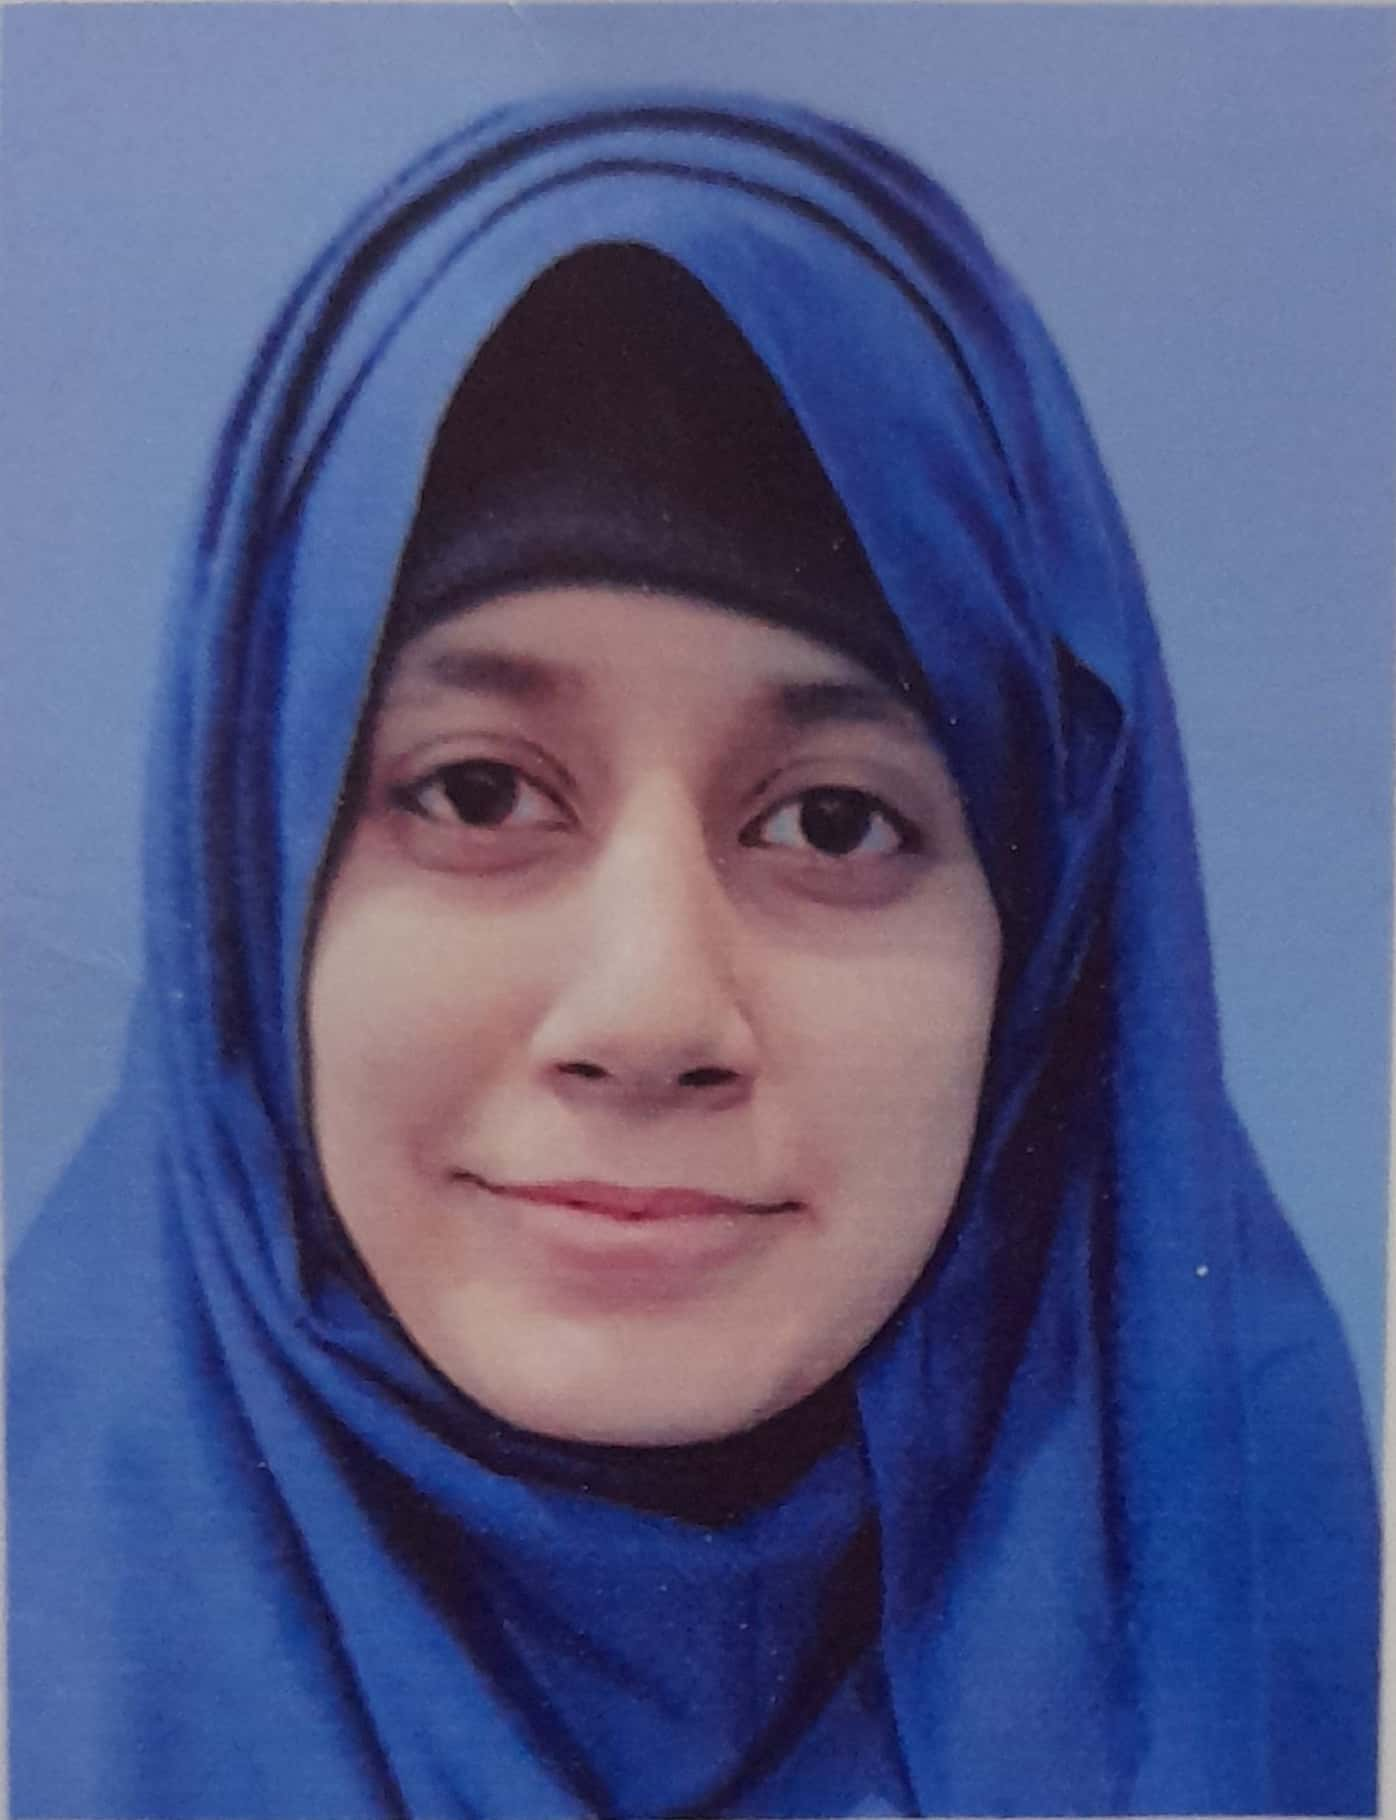
\includegraphics[width=2.5cm,height=3.2cm]{image.jpg}
\end{column}

\end{multicols}

\vspace{10pt}

% Skills section

{\Large \textbf{Skills:}}
\begin{itemize}
    \item \textbf{Machine Learning:} Regression, Classification, Decision Trees, Random Forests, SVM, Neural Networks
    \item \textbf{Deep Learning:} TensorFlow, PyTorch
    \item \textbf{Natural Language Processing:} Text Classification, Sentiment Analysis, NER
    \item \textbf{Computer Vision:} Image Classification, Object Detection, Segmentation
    \item \textbf{Data Preprocessing:} Cleaning, Transformation, Feature Engineering
    \item \textbf{Programming:} Python, SQL, C++
\end{itemize}


% Work Experience section
\vspace{10pt}
{\Large \textbf{Work Experience:}} % Section title made larger and bold

\textbf{August 2024 - Present} \hfill \textbf{National University of Computer and Emerging Sciences} \hfill Pakistan\\
\textit{Teaching Assistant}
\begin{itemize}
    \item Teaching Assistant for Programming Fundamentals - Fall 2024
    \item Teaching Assistant for Computer Organization And Assembly Language - Fall 2024
    \item Assisted in creating and grading AI-related assignments and projects.
    \item Supported students in implementing machine learning and AI algorithms.
\end{itemize}

\vspace{5pt}
\textbf{July 2024 - August 2024} \hfill \textbf{Tech Innovators} \hfill Pakistan \\
\textit{AI Research and Development Intern}
\begin{itemize}
    \item Researched and developed advanced AI algorithms for predictive analytics and computer vision tasks.
    \item Implemented a state-of-the-art object detection model using a deep learning framework to improve image recognition accuracy.
    \item Collaborated with a cross-functional team to integrate machine learning models into a real-time application for efficient decision-making.
\end{itemize}
% Education section
\vspace{10pt}
{\Large \textbf{Education:}} % Section title made larger and bold

\textbf{2022 - 2026} \hfill \textbf{National University of Computer and Emerging Sciences} \hfill Pakistan\\
\textit{Bachelor of Science - BS, Artificial Intelligence}

\textbf{August 2020 - August 2022} \hfill \textbf{Hadaf Group of Colleges Peshawar} \hfill Pakistan\\
\textit{FSc, Pre-Engineering}

% Projects section
\vspace{10pt}
{\Large \textbf{Projects:}} % Section title made larger and bold
\begin{itemize}
    \item \textbf{Book Recommendation System using FP-growth algorithm} (Sep 2024)
    \item \textbf{Expense App} (Jul 2024 - Aug 2024)
    \item \textbf{University Management System and Student Services} (May 2024 - Jun 2024)
    \item \textbf{Pneumonia Detection} (Mar 2024 - May 2024)
\end{itemize}


% Certifications section
\vspace{10pt}
{\Large \textbf{Certifications:}} % Section title made larger and bold
\begin{itemize}
    \item Programming for Everybody (Getting Started with Python)
    \item Python Data Structures
    \item Responsive Web Design
    \item Simple Linear Regression for the Absolute Beginner
\end{itemize}

\end{document}
% }}}}